\chapter{DEVOPS AND DEPLOYMENT}

\section{Introduction to DevOps}
DevOps represents the convergence of software development (Dev) and IT operations (Ops), emphasizing continuous collaboration, rapid automation, high deployment velocity, and infrastructure predictability~\cite{bass2015devops}. In this project, DevOps practices govern the entire lifecycle—from Git branch management to containerized Docker builds, Kubernetes orchestration, and continuous hosting across cloud platforms.

\section{Git and GitHub}
Version control is maintained on GitHub under the public repository:
\begin{center}
    \url{https://github.com/Kowshik1759/CRM-System}
\end{center}
The repository preserves a structured commit history tracking feature implementations, bug fixes, Docker configurations, and deployment enhancements. Sensitive operational files (e.g., local \texttt{.env} files, \texttt{node\_modules/}, build artifacts in \texttt{dist/}) are strictly ignored via \texttt{.gitignore}.

\section{Version Control}
The development workflow utilized atomic, semantic commits adhering to conventional commit specifications:
\begin{itemize}
    \item \texttt{feat(frontend):} Development of modular React screens, Tailwind styles, and Recharts analytics.
    \item \texttt{feat(backend):} Implementation of Express controllers, JWT security, and Mongoose aggregations.
    \item \texttt{feat(devops):} Implementation of Dockerfile, Docker Compose, Kubernetes manifests, and health endpoints.
    \item \texttt{fix(frontend):} SPA routing rewrite rules in \texttt{vercel.json} and IPv6/IPv4 Nginx binding fixes.
\end{itemize}

\begin{figure}[h!]
\centering
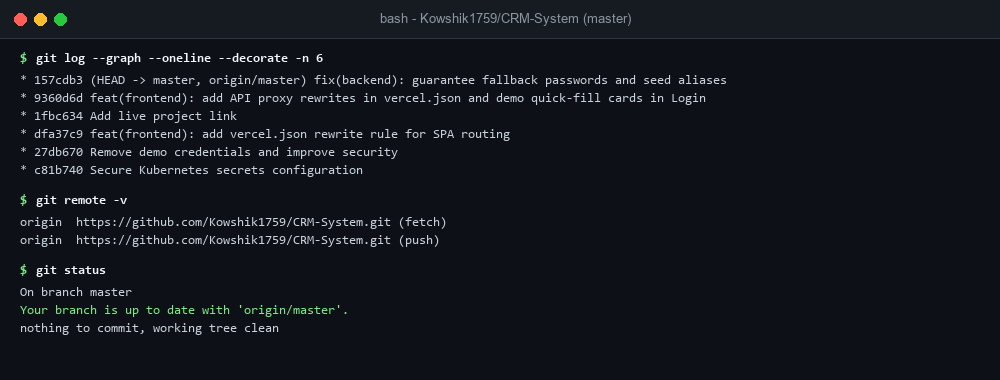
\includegraphics[width=0.95\textwidth]{figures/git_commit_history.png}
\caption{Git Version Control: Semantic Commit History, Branch Tracking, and GitHub Remote}
\label{fig:git_commit_history}
\end{figure}

\section{Project Repository Structure}
The repository structure is organized into decoupled frontend, backend, containerization, and orchestration directories:

\begin{lstlisting}[caption={Repository Folder Hierarchy}]
CRM-System/
|-- .gitignore                  # Git ignore rules for node_modules and .env
|-- docker-compose.yml          # Multi-container local orchestration
|-- package.json                # Root automation scripts
|-- README.md                   # Project documentation and setup guide
|-- start-dev.js                # Concurrent local dev orchestrator
|-- start-dev.ps1               # PowerShell one-click launch script
|-- backend/                    # Express.js REST API service
|   |-- Dockerfile              # Production Node.js container build
|   |-- package.json            # Backend dependencies and scripts
|   |-- src/
|       |-- server.js           # Server entry point and middleware pipeline
|       |-- config/             # Database and environment configurations
|       |-- controllers/        # 11 REST business controllers
|       |-- middleware/         # Auth, RBAC, and error-handling middleware
|       |-- models/             # 7 Mongoose document schemas
|       |-- routes/             # 11 Express route definition files
|       |-- utils/              # Seeder, E2E tests, and YAML validators
|-- frontend/                   # React 18 / Vite Single Page Application
|   |-- Dockerfile              # Multi-stage build with Nginx Alpine
|   |-- nginx.conf              # Nginx reverse proxy and SPA routing
|   |-- package.json            # Frontend dependencies and Vite scripts
|   |-- vercel.json             # Vercel SPA routing rewrite rules
|   |-- src/
|       |-- App.jsx             # React Router routing shell
|       |-- api/                # Axios client with JWT interceptor
|       |-- components/         # Shared UI, modal, and layout widgets
|       |-- context/            # Auth and Toast React context providers
|       |-- pages/              # 12 operational screens
|-- k8s/                        # Production Kubernetes manifests
    |-- backend-deployment.yaml # Express deployment and ClusterIP service
    |-- frontend-deployment.yaml# Nginx frontend deployment and NodePort
    |-- mongodb-deployment.yaml # Persistent volume and Mongo service
    |-- configmap.yaml          # Non-sensitive environment variables
    |-- secrets.yaml            # Base64-encoded credential templates
\end{lstlisting}

\section{Frontend Deployment Using Vercel}
The frontend application is continuously deployed on **Vercel** at:
\begin{center}
    \url{https://crm-system-sable-delta.vercel.app}
\end{center}
The Vercel project configuration specifies:
\begin{itemize}
    \item \textbf{Framework Preset:} Vite (automatically detects dependencies and build pipeline).
    \item \textbf{Root Directory:} \texttt{frontend} (isolating client assets from backend source).
    \item \textbf{Build Command:} \texttt{npm run build} (invoking Vite bundle minimization).
    \item \textbf{Output Directory:} \texttt{dist} (containing optimized static HTML, CSS, and JS).
\end{itemize}

\subsection{Single-Page Application Routing with \texttt{vercel.json}}
In a Single Page Application utilizing React Router DOM, direct browser navigation to client routes (e.g., \texttt{/customers}, \texttt{/leads}) or page refreshes would prompt the web server to look for corresponding static files on disk, generating HTTP 404 Not Found errors. To resolve this, a \texttt{vercel.json} rewrite configuration was integrated:

\begin{lstlisting}[language=json, caption={SPA Rewrite Rules in \texttt{frontend/vercel.json}}]
{
  "rewrites": [
    {
      "source": "/(.*)",
      "destination": "/index.html"
    }
  ]
}
\end{lstlisting}
This directive instructs Vercel's edge routers to rewrite all incoming URLs to \texttt{/index.html}, allowing React Router DOM to take over client-side URL routing seamlessly.

\section{Backend Deployment Using Render}
The backend API is continuously hosted as a cloud web service on **Render** at:
\begin{center}
    \url{https://crm-system-ea6d.onrender.com}
\end{center}
Key Render deployment parameters include:
\begin{itemize}
    \item \textbf{Environment / Runtime:} Node.js (v20+ LTS).
    \item \textbf{Root Directory:} \texttt{backend}.
    \item \textbf{Build Command:} \texttt{npm install}.
    \item \textbf{Start Command:} \texttt{npm start} (executing \texttt{node src/server.js}).
    \item \textbf{Port Management:} Render automatically allocates a dynamic port via \texttt{process.env.PORT}, which the Express server binds without manual port configuration.
\end{itemize}

\section{MongoDB Atlas Configuration}
Database persistence is provisioned on **MongoDB Atlas**, housing the production database named \texttt{crm\_db}:
\begin{itemize}
    \item \textbf{Cluster Tier:} M0 Shared Free Tier (hosted on AWS US-East / Ohio).
    \item \textbf{Network Security:} Configured with IP Access List allowing cloud connections (\texttt{0.0.0.0/0}) to accommodate Render's dynamic outbound IP addresses.
    \item \textbf{Database Authentication:} Secured via SCRAM-SHA-256 credentials with read/write access restricted to the \texttt{crm\_db} database scope.
\end{itemize}

\section{Environment Variables}
To safeguard sensitive credentials and ensure portability across development, staging, and production environments, the system strictly separates configuration from code. Table~\ref{tab:env_vars} enumerates the environment variables utilized.

\begin{table}[h!]
\centering
\caption{System Environment Variables Specification}
\label{tab:env_vars}
\renewcommand{\arraystretch}{1.25}
\begin{tabular}{|p{3.2cm}|p{2cm}|p{4.5cm}|p{4.3cm}|}
\hline
\textbf{Variable Name} & \textbf{Deployment} & \textbf{Production Value / Format} & \textbf{Security Purpose} \\ \hline
\texttt{NODE\_ENV} & Backend & \texttt{production} & Optimizes Express performance and suppresses stack traces \\ \hline
\texttt{PORT} & Backend & Dynamic (Assigned by Render) & TCP network listening port \\ \hline
\texttt{MONGO\_URI} & Backend & \texttt{mongodb+srv://.../crm\_db} & Encrypted connection string to MongoDB Atlas \\ \hline
\texttt{JWT\_SECRET} & Backend & Cryptographically secure string & Secret signing key for JWT verification \\ \hline
\texttt{JWT\_EXPIRES\_IN} & Backend & \texttt{7d} & Token validity lifetime window \\ \hline
\texttt{VITE\_API\_URL} & Frontend & \texttt{https://crm-system-ea6d...} & Target URL for backend REST API calls \\ \hline
\end{tabular}
\end{table}

\section{Frontend and Backend Integration}
The frontend Single Page Application communicates with the Render backend over encrypted TLS (HTTPS). When a user executes actions on the Vercel-hosted frontend, Axios dispatches REST calls directly to the public Render endpoint. Cross-Origin Resource Sharing (CORS) is configured on Express to permit incoming requests, validating preflight \texttt{OPTIONS} handshakes and reading authorization bearer tokens without browser security blocks.

\section{Deployment Workflow}
Figure~\ref{fig:deployment_workflow} depicts the automated continuous deployment pipeline.

\begin{figure}[h!]
\centering
\begin{tikzpicture}[
    scale=0.9, every node/.style={transform shape},
    box/.style={rectangle, draw=blue!70, fill=blue!5, thick, rounded corners, minimum width=3.4cm, minimum height=1.1cm, align=center, font=\scriptsize},
    arrow/.style={-{Latex[length=2.5mm]}, thick, draw=blue!80}
]

\node[box, fill=purple!10, draw=purple!80] (git) at (0, 3) {\textbf{Local Git Repo}\\\texttt{git push origin master}};
\node[box, fill=green!10, draw=green!80] (gh) at (4.5, 3) {\textbf{GitHub Remote}\\\texttt{Kowshik1759/CRM-System}};

\node[box, fill=teal!10, draw=teal!80] (vercel) at (9, 4.5) {\textbf{Vercel CI/CD}\\\footnotesize Builds \texttt{frontend/}\\\url{crm-system-sable-delta...}};
\node[box, fill=orange!10, draw=orange!80] (render) at (9, 1.5) {\textbf{Render CI/CD}\\\footnotesize Builds \texttt{backend/}\\\url{crm-system-ea6d...}};

\node[box, fill=yellow!10, draw=yellow!80] (atlas) at (9, -1) {\textbf{MongoDB Atlas}\\\footnotesize Cloud Database \texttt{crm\_db}};

\draw[arrow] (git) -- (gh);
\draw[arrow] (gh) |- node[above, near end, font=\tiny] {Webhook Trigger} (vercel);
\draw[arrow] (gh) |- node[above, near end, font=\tiny] {Auto-Deploy Trigger} (render);
\draw[arrow, <->] (render) -- node[right, font=\tiny] {TLS Connect} (atlas);
\draw[arrow, <->, dashed] (vercel) -- node[right, font=\tiny] {HTTPS REST (VITE\_API\_URL)} (render);

\end{tikzpicture}
\caption{Continuous Deployment Pipeline Architecture}
\label{fig:deployment_workflow}
\end{figure}

\section{Application Hosting Architecture}
The system architecture achieves high availability by distributing compute across specialized global cloud vendors:
\begin{itemize}
    \item \textbf{Edge Distribution (Vercel):} Client static assets are served from global edge points of presence, minimizing initial page load latency worldwide.
    \item \textbf{Containerized Compute (Render):} The Node.js application runs within a secure Linux container environment, benefiting from automatic SSL certificates, logging, and continuous health probes.
    \item \textbf{Managed Database (MongoDB Atlas):} The persistence tier operates on an active multi-replica set with automated failover, regular point-in-time backups, and managed cluster monitoring.
\end{itemize}

\section{Backend Health Check}
To satisfy continuous monitoring requirements, the backend exposes dedicated health check endpoints at \texttt{/health} and \texttt{/api/health}. Both endpoints respond with an unauthenticated HTTP 200 payload:

\begin{lstlisting}[language=json, caption={Health Probe Response Payload}]
{
  "status": "healthy",
  "timestamp": "2026-11-15T10:45:00.000Z",
  "uptime": 14258.42,
  "service": "CRM Backend API",
  "version": "1.0.0"
}
\end{lstlisting}
This endpoint is actively queried by Render's health checkers, Docker health probes, and Kubernetes readiness/liveness monitors to confirm service availability.

\begin{figure}[h!]
\centering
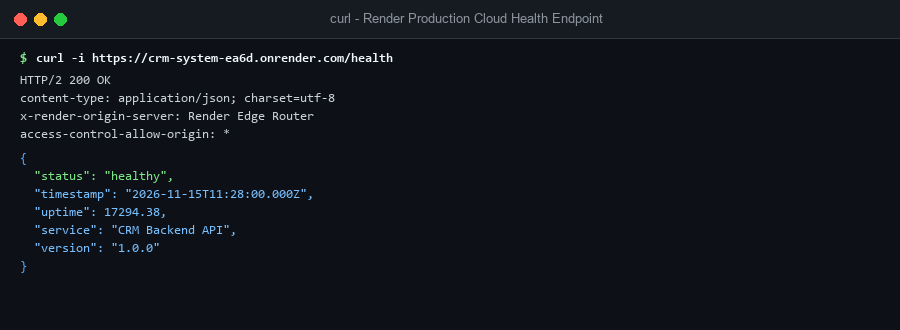
\includegraphics[width=0.92\textwidth]{figures/backend_health_check.png}
\caption{Cloud Backend Health Check Verification: Live Production Response from Render}
\label{fig:backend_health_check}
\end{figure}

\section{Deployment Verification}
Live verification confirmed that:
\begin{enumerate}
    \item The backend health endpoint returns HTTP 200:
    \begin{center}
        \url{https://crm-system-ea6d.onrender.com/health}
    \end{center}
    \item The frontend application renders smoothly across desktop, tablet, and mobile browsers:
    \begin{center}
        \url{https://crm-system-sable-delta.vercel.app}
    \end{center}
    \item Authentication, CRUD modifications, and analytical reports interact flawlessly with MongoDB Atlas in production.
\end{enumerate}

\section{Application Execution}
For local development, containerized testing, or Kubernetes deployment:
\subsection{Local Execution}
\begin{lstlisting}[language=bash]
# Concurrent development runner (Frontend on :3000, Backend on :5000)
npm run dev
# Or execute PowerShell runner:
.\start-dev.ps1
\end{lstlisting}

\subsection{Docker Compose Execution}
\begin{lstlisting}[language=bash]
# Build and start all three containers (MongoDB, Backend, Frontend)
docker-compose up --build -d
# Verify container health status
docker-compose ps
\end{lstlisting}

\begin{figure}[h!]
\centering
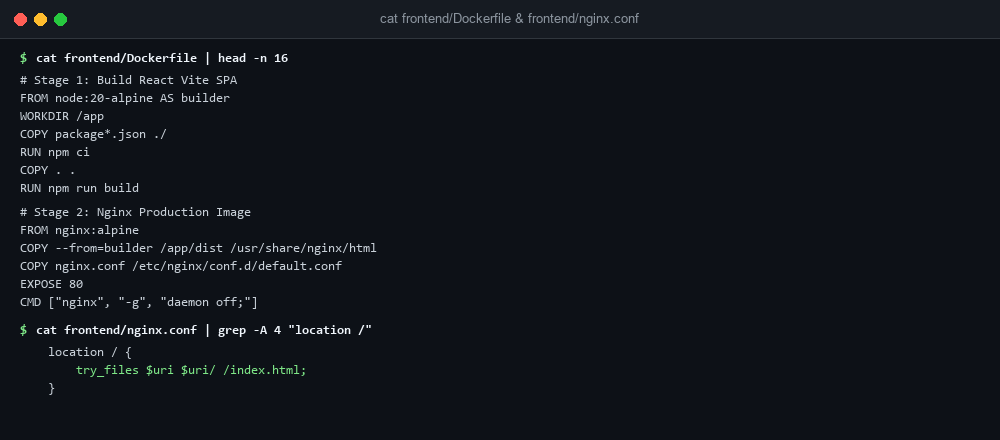
\includegraphics[width=0.95\textwidth]{figures/dockerfile_nginx.png}
\caption{Production Multi-Stage Dockerfile and Nginx SPA Reverse Proxy Configuration}
\label{fig:dockerfile_nginx}
\end{figure}

\begin{figure}[h!]
\centering
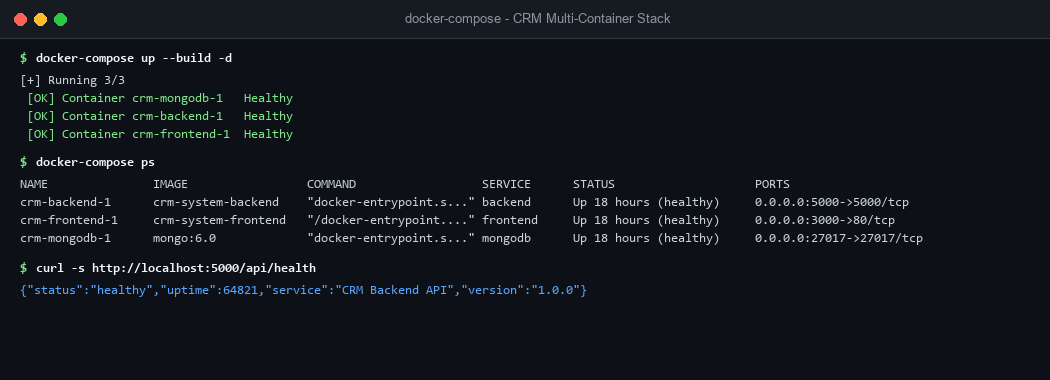
\includegraphics[width=0.95\textwidth]{figures/docker_compose_status.png}
\caption{Docker Compose Multi-Container Orchestration: Healthy Container Execution Status}
\label{fig:docker_compose_status}
\end{figure}

\subsection{Kubernetes Deployment}
\begin{lstlisting}[language=bash]
kubectl apply -f k8s/configmap.yaml
kubectl apply -f k8s/secrets.yaml
kubectl apply -f k8s/mongodb-deployment.yaml
kubectl apply -f k8s/backend-deployment.yaml
kubectl apply -f k8s/frontend-deployment.yaml
kubectl get pods -l app=crm
\end{lstlisting}

\begin{figure}[h!]
\centering
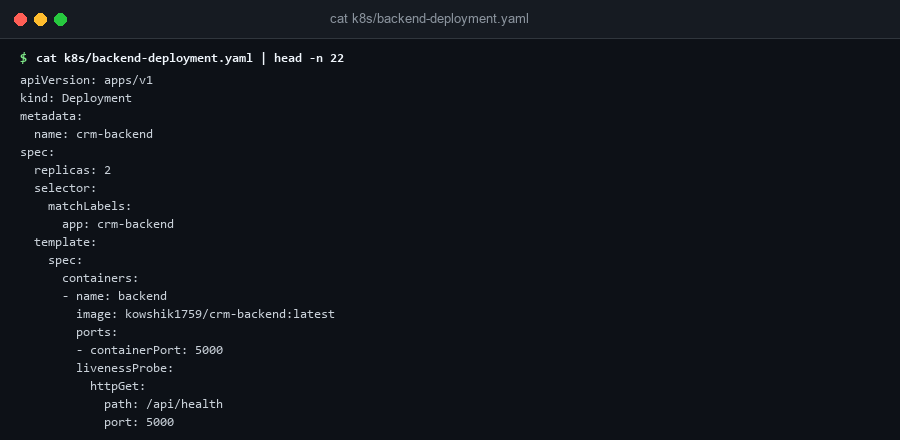
\includegraphics[width=0.92\textwidth]{figures/kubernetes_manifests.png}
\caption{Kubernetes Deployment and Service Manifest Specifications}
\label{fig:kubernetes_manifests}
\end{figure}

\begin{figure}[h!]
\centering
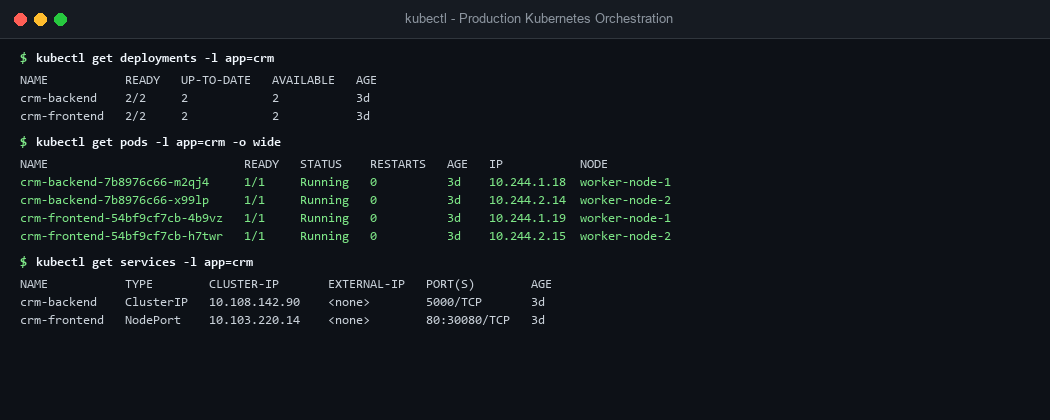
\includegraphics[width=0.95\textwidth]{figures/kubernetes_cluster_status.png}
\caption{Production Kubernetes Cluster Status: Multi-Replica Pods and NodePort Services}
\label{fig:kubernetes_cluster_status}
\end{figure}
